% \section{Method}
\section{多视角3D目标检测}
\subsection{概述}
\label{overview}
% Talk about the pipeline in high level and why our method is exciting. 
% We consider an application of 3D object detection where the scene geometry is missing and only 2D multi-camera images are available. This challenging problem gives rise to  . 

本文架构以一组相机（其投影矩阵已知）采集的RGB图像作为输入，输出场景中目标的3D边界框参数集合。与以往方法不同，本文基于以下几个高层次需求构建架构：
\begin{itemize}
    \item 在架构的中间计算中融入3D信息，而非仅在图像平面上执行纯2D计算。
    \item 不估计密集的3D场景几何结构，避免引入相关的重建误差。
    \item 避免NMS等后处理步骤。
\end{itemize}

\begin{figure}[t!]  
    \centering
    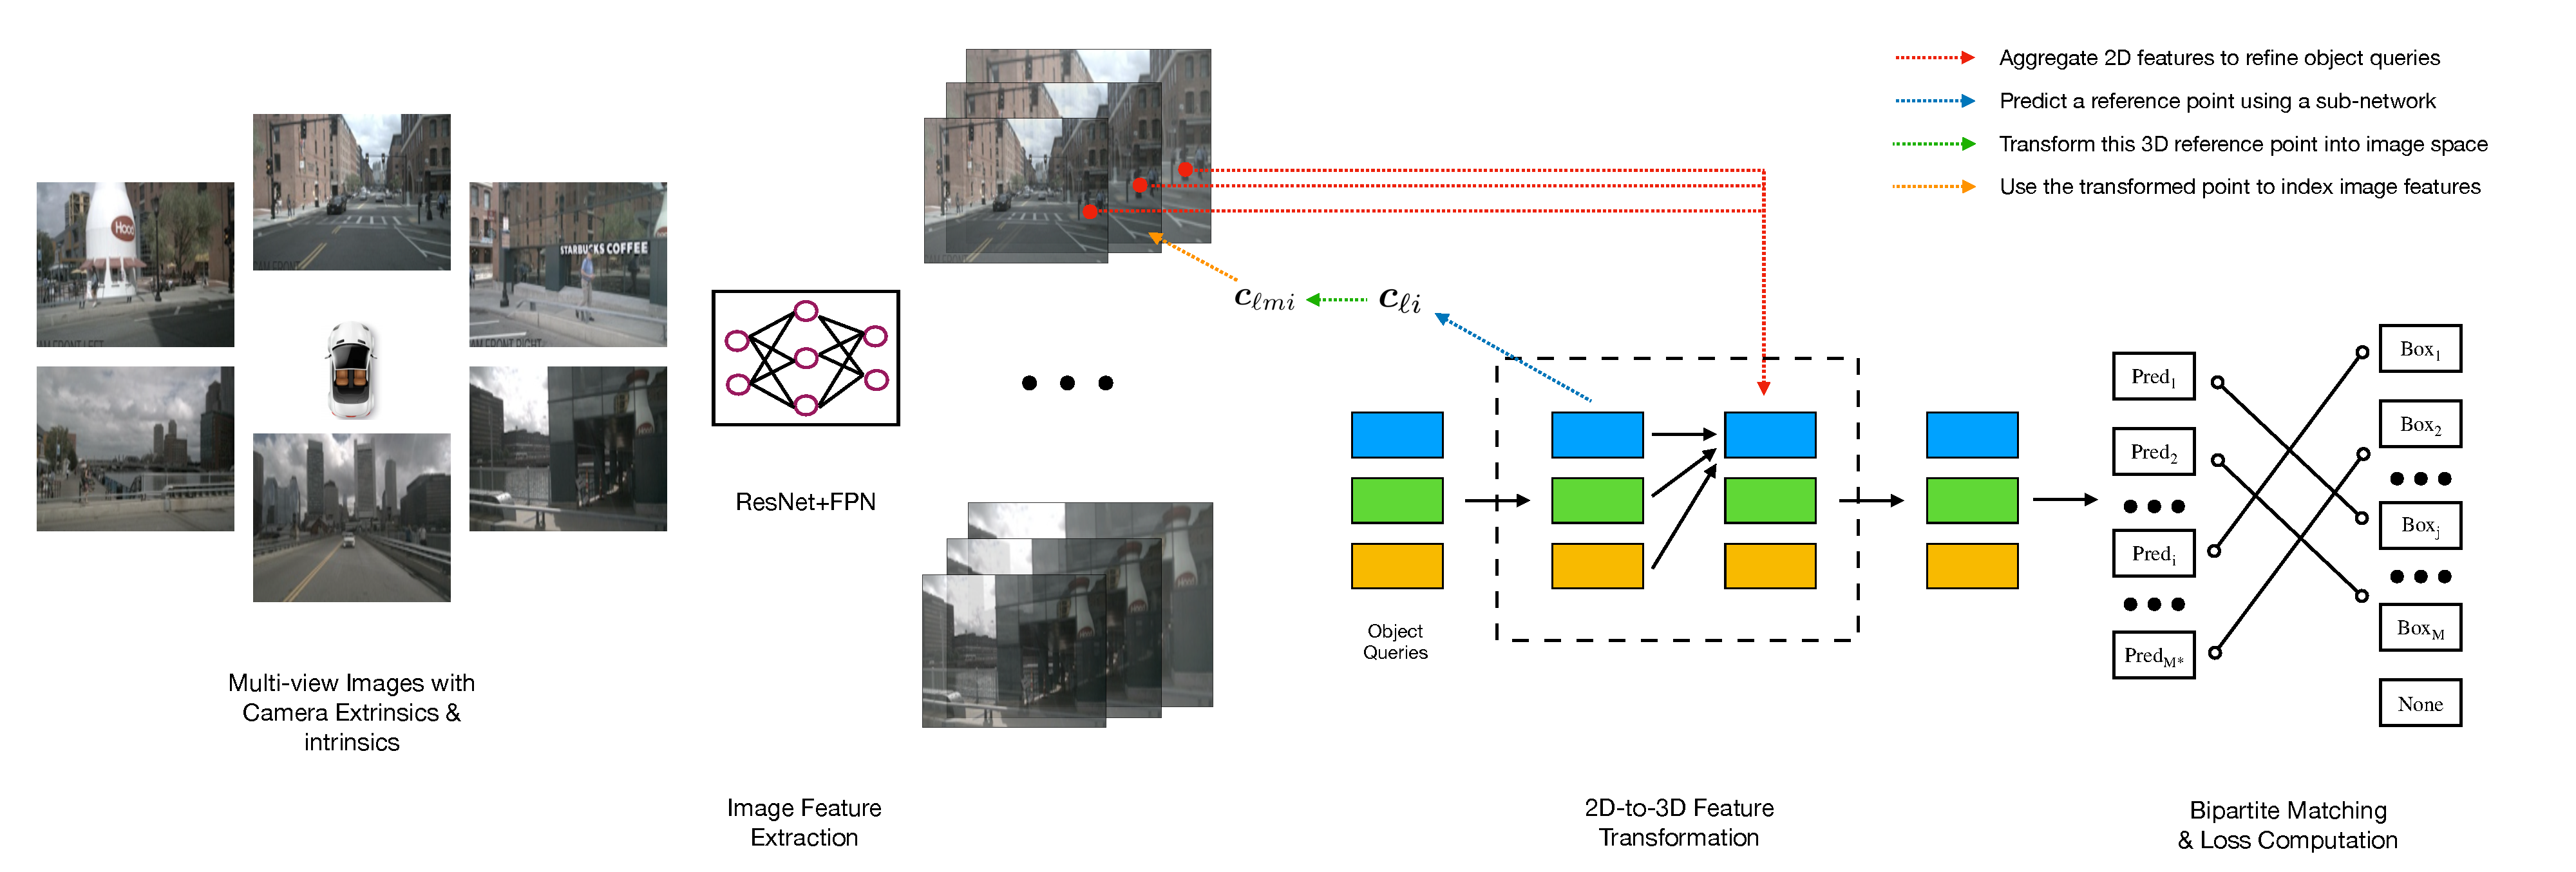
\includegraphics[width=1.0\columnwidth]{figure/architecture}
    \vspace{-1em}
  \caption{本文方法概述。模型输入为一组多视角图像，经ResNet和FPN编码后，模型在一组稀疏的目标查询上操作，每个查询解码为一个3D参考点。通过将3D参考点投影到图像空间，提取2D特征以优化目标查询。模型对每个查询进行预测，并使用集合到集合损失。\label{fig:architecture}}
  \vspace{-2em}
\end{figure}

本文通过一个新的集合预测模块满足这些需求，该模块在2D和3D计算之间交替，连接2D特征提取与3D框预测。模型包含三个关键组件，如图~\ref{fig:architecture}所示。首先，遵循2D视觉中的常见做法，使用共享的ResNet~\cite{He2015}骨干网络从相机图像中提取特征，并可选地使用特征金字塔网络（Feature Pyramid Network, FPN）~\cite{Lin2017}增强这些特征（\S\ref{feature-learning}）。其次，检测头（\S\ref{detection-head}）——本文的主要贡献——以几何感知的方式将计算得到的2D特征与一组3D边界框预测连接起来（\S\ref{detection-head}）。检测头的每一层从一组稀疏的目标查询开始，这些查询从数据中学习得到。每个目标查询编码一个3D位置，该位置被投影到相机平面并通过双线性插值收集图像特征。与DETR~\cite{detr}类似，使用多头注意力~\cite{Vaswani2017}通过融入目标交互来优化目标查询。该层重复多次，在特征采样和目标查询优化之间交替。最后，使用集合到集合损失~\cite{StewartAN16,detr}训练网络（\S\ref{loss}）。

\subsection{特征学习}
\label{feature-learning}
模型以一组图像 $\I=\{\mathrm{\mathbf{im}}_1, \ldots, \mathrm{\mathbf{im}}_K\} \subset\R^{\mathrm{H_{im}}\times \mathrm{W_{im}}\times3}$（由环视相机拍摄）、相机矩阵 $\T=\{T_1, \ldots, T_K\} \subset \R^{3\times4}$、真值边界框 $\B=\{\bb_1, \ldots, \bb_j, \ldots, \bb_M\}\subset\R^9$ 和类别标签 $\C = \{c_1, \ldots, c_j, \ldots, c_M\}\subset\mathbb{Z}$ 为输入。每个 $\bb_j$ 包含在鸟瞰视图（Bird's-Eye View, BEV）中的位置、尺寸、朝向角和速度；本文旨在从图像中预测这些边界框及其标签。本文\emph{不}使用通常由高端激光雷达捕获的点云。

% \justin{fix the 4,  6 constants ``hard coded'' below---move those to experiments and use letters}
这些图像经ResNet~\cite{He2015}和FPN~\cite{Lin2017}编码为四组特征 $\F_1, \F_2, \F_3, \F_4$。每组特征 $\F_k=\{\bff_{k1}, \ldots, \bff_{k6}\} \subset \R^{H\times W \times C}$ 对应6张图像的一个特征层级。这些多尺度特征提供了丰富的信息，以识别不同大小的目标。下面详细阐述如何通过新颖的集合预测模块将这些2D特征转换为3D特征。

% \subsection{Object Queries}
% \label{object-query}

\subsection{检测头}
\label{detection-head}

现有的从相机输入进行目标检测的方法通常采用自底向上的方式，即对每张图像预测一组密集的边界框，在图像间过滤冗余框，并在后处理步骤中聚合所有相机的预测。该范式有两个关键缺陷：密集边界框预测需要准确的深度感知（这本身就是一个具有挑战性的问题）；基于NMS的冗余去除和聚合是不可并行化的操作，会引入显著的推理开销。本文通过下面描述的自顶向下检测头来解决这些问题。

与~\cite{objdgcnn, zhu2021deformable}类似，\name 是\emph{迭代式}的；使用 $L$ 层基于集合的计算从2D特征图中生成边界框估计。每一层包括以下步骤：
\begin{enumerate}
    \item 预测与目标查询关联的一组边界框中心；
    \item 使用相机变换矩阵将这些中心投影到所有特征图中；
    \item 通过双线性插值采样特征并将其融入目标查询；
    \item 使用多头注意力描述目标交互。
\end{enumerate}

受DETR~\cite{detr}启发，每一层 $\ell\in\{0,\ldots,L-1\}$ 对一组\emph{目标查询} $\Q_\ell=\{\bq_{\ell 1}, \ldots, \bq_{\ell M^*}\}\subset\R^{C}$ 进行操作，生成新集合 $\Q_{\ell+1}$。从目标查询 $\bq_{\ell i}$ 解码出参考点 $\bc_{\ell i}\in \R^3$：
\begin{equation}\label{eq:query-point}
    \begin{split}
      \bc_{\ell i}=\Phi^{\mathrm{ref}}(\bq_{\ell i}),
    \end{split}
\end{equation}
其中 $\Phi^{\mathrm{ref}}$ 是一个神经网络。$\bc_{\ell i}$ 可视为第 $i$ 个框中心的一个假设。接下来，获取与 $\bc_{\ell i}$ 对应的图像特征，以优化并预测最终的边界框。然后，使用相机变换矩阵将 $\bc_{\ell i}$（更准确地说，其齐次坐标 $\bc_{\ell i}^*$）投影到每张图像中：
\begin{equation}\label{eq:point-projection}
    \begin{split}
      \bc_{\ell i}^* = \bc_{\ell i} \oplus 1 \qquad\qquad \bc_{\ell m i} = T_m \bc_{\ell i}^*,
    \end{split}
\end{equation}
其中 $\oplus$ 表示拼接操作，$\bc_{\ell m i}$ 是参考点在第 $m$ 个相机上的投影。为消除特征图大小的影响并收集不同层级的特征，将 $\bc_{\ell m i}$ 归一化到 $[-1, 1]$。接下来，通过以下方式收集图像特征：
\begin{equation}\label{eq:bilinear}
    \begin{split}
        \bff_{\ell k m i}  = f^{\mathrm{bilinear}}(\F_{km}, \bc_{\ell m i}),
    \end{split}
\end{equation}
其中 $\bff_{\ell k m i}$ 是第 $\ell$ 层中第 $i$ 个点在第 $m$ 个相机第 $k$ 个特征层级上的特征。

给定参考点不一定在所有相机图像中都可见，因此需要使用启发式方法过滤无效点。为此，定义二值变量 $\sigma_{\ell k m i}$，其取值基于参考点是否投影到图像平面之外。最终特征 $\bff_{\ell i}$ 和下一层的目标查询 $\bq_{(\ell+1) i}$ 由下式给出：
\begin{equation}\label{eq:feature-agg}
    \begin{split}
        \bff_{\ell i}  = \frac{1}{\sum_k\sum_m \sigma_{\ell k m i}+\epsilon}\sum_k \sum_m \bff_{\ell k m i} \sigma_{\ell k m i} \qquad \mathrm{and} \qquad \bq_{(\ell+1)i} = \bff_{\ell i}  + \bq_{\ell i},
    \end{split}
\end{equation}
其中 $\epsilon$ 是一个微小数值，用于避免除零。最后，对每个目标查询 $\bq_{\ell i}$，使用两个神经网络 $\Phi_{\ell}^{\mathrm{reg}}$ 和 $\Phi_{\ell}^{\mathrm{cls}}$ 预测边界框 $\hat{\bb}_{\ell i}$ 及其类别标签 $\hat{c}_{\ell i}$：
\begin{equation}\label{eq:prediction}
    \begin{split}
      \hat{\bb}_{\ell i} = \Phi_{\ell}^{\mathrm{reg}}(\bq_{\ell i})  \qquad \mathrm{and} \qquad   \hat{c}_{\ell i} = \Phi_{\ell}^{\mathrm{cls}}(\bq_{\ell i}).
    \end{split}
\end{equation}
在训练期间，对每一层的预测 $\hat{\B}_\ell =\{\hat{\bb}_{\ell 1}, \ldots, \hat{\bb}_{\ell j}, \ldots, \hat{\bb}_{\ell M^\ast}\}\subset\R^9$ 和 $\hat{\C}_\ell = \{\hat{c}_{\ell 1}, \ldots, \hat{c}_{\ell j}, \ldots, \hat{c}_{\ell M}\}\subset\mathbb{Z}$ 计算损失。推理时，只使用最后一层的输出。
% \justin{Something seems to be missing here.  Do you define how you obtain $\B,\C$ used in the next section.  Make sure every step is clear here.  Also, where do you predict the \emph{number} of boxes in the scene?}

\subsection{损失函数}
\label{loss}

参考~\cite{StewartAN16,detr}，使用集合到集合损失来衡量预测集合 $(\hat{\B}_\ell, \hat{\C}_\ell)$ 与真值集合 $(\B, \C)$ 之间的差异。该损失由两部分组成：类别标签的焦点损失（Focal Loss）~\cite{lin2017focal}和边界框参数的 $L^1$ 损失。为书写方便，省略 $\hat{\B}_\ell$ 和 $\hat{\C}_\ell$ 中的下标 $\ell$。真值框的数量 $M$ 通常小于预测数量 $M^\ast$，因此将真值框集合用 $\varnothing$（无目标）填充到 $M^{\ast}$ 以便于计算。通过二分匹配（Bipartite Matching）问题建立真值与预测之间的对应关系：$\sigma^{\ast} = \argmin_{\sigma \in \mathcal{P}}\sum_{j=1}^M -1_{\{c_j\neq\varnothing\}}\hat{p}_{\sigma(j)}(c_j) + 1_{\{c_j=\varnothing\}}\mathcal{L}_{\mathrm{box}}(\bb_j, \hat{\bb}_{\sigma(j)}),$

其中 $\mathcal{P}$ 表示所有排列的集合，$\hat{p}_{\sigma(j)}(c_j)$ 是索引 $\sigma(j)$ 的预测属于类别 $c_j$ 的概率，$\mathcal{L}_{\mathrm{box}}$ 是边界框参数的 $L_1$ 损失。与~\cite{StewartAN16,detr}一样，使用匈牙利算法~\cite{Kuhn55thehungarian}求解该分配问题，得到集合到集合损失 $\mathcal{L_{\mathrm{sup}}} = \sum_{j=1}^N -\log\hat{p}_{\sigma^{\ast}(j)}(c_j) + 1_{\{c_j=\varnothing\}}\mathcal{L}_{\mathrm{box}}(\bb_j, \hat{\bb}_{\sigma^{\ast}(j)})$.
% \begin{equation}\label{eq:sup_loss}
%      \begin{split}
%       \mathcal{L_{\mathrm{sup}}} = \sum_{j=1}^N -\log\hat{p}_{\sigma^{\ast}(j)}(c_j) + 1_{\{c_j=\varnothing\}}\mathcal{L}_{\mathrm{box}}(\bb_j, \hat{\bb}_{\sigma^{\ast}(j)}).
%      \end{split}
% \end{equation}



